\subsection{Caso 4. Detección de anomalías con IA/ML en tráfico TCP/IP}
\label{caso:anomalias-ml}

\begin{situacion}
El equipo debe proponer una defensa inteligente que identifique desviaciones frente al tráfico normal.

\textbf{Objetivo:} \par
Construir y evaluar una línea base estadística y un detector de anomalías basado en Isolation Forest para identificar desviaciones del tráfico TCP/IP, separando temporalmente el entrenamiento de la evaluación y considerando los falsos positivos producidos por cambios legítimos de carga. \par

\textbf{Fundamento teórico:} \par
La línea base estadística estandariza los atributos respecto al tráfico benigno y marca como anómala una ventana cuyo máximo valor absoluto de \textit{z-score} supera el umbral de tres desviaciones estándar. Isolation Forest construye particiones aleatorias de los atributos y asigna puntuaciones más altas a las observaciones que se aíslan con mayor facilidad \parencite{liu2008isolation,sklearn}. En ambos casos es necesario evitar la fuga de datos: el escalado, el entrenamiento y la calibración del umbral no deben utilizar información del conjunto de prueba.

El desbalance de clases hace que la precisión, el recall, la F1, la PR-AUC y la tasa de falsos positivos sean más informativas que una exactitud global aislada. La deriva de concepto aparece cuando el tráfico legítimo cambia de distribución, como ocurre con una ráfaga autorizada; por ello, una detección debe persistir durante varias ventanas y mantenerse bajo revisión humana.
\end{situacion}

\paragraph{Procedimiento.}
La plantilla original conserva cuatro actividades: crear atributos agregados, separar temporalmente los datos para evitar fuga, comparar la línea base con un detector de anomalías y proteger los ejemplos de entrenamiento. En el artefacto evaluado, los tamaños documentados son \texttt{n\_train}=540, \texttt{n\_validation}=90 y \texttt{n\_test}=363, según se registra en \texttt{laboratorio/work/cu4/metricas.json}.

\begin{enumerate}
\item \textbf{Custodia e integridad:} se preparó la evidencia de las capturas PCAP (\texttt{CU4\_01\_benign.pcap}, \texttt{CU4\_02\_flash\_crowd.pcap} y \texttt{CU4\_03\_synflood\_attack.pcap}) y su comprobación de integridad mediante la verificación de hashes SHA-256. La evidencia gráfica asociada se presenta en la Figura~\ref{fig:c4_hashes}.
\item \textbf{Línea base benigna y ráfaga legítima:} se incorporaron ventanas benignas y una condición de cambio legítimo de carga (\textit{flash crowd}). El análisis dividió el tráfico en 540 ventanas de entrenamiento benigno, 90 de validación y 363 de prueba. Se creó un conjunto de datos con características agregadas: conexiones por minuto, bytes por flujo, duración, flags TCP y proporción petición/respuesta.
\item \textbf{Extracción de atributos:} \texttt{analyze\_cu4.py} calculó por ventana temporal de 1 segundo los atributos \texttt{conns\_per\_min}, \texttt{bytes\_per\_flow}, \texttt{flow\_duration}, \texttt{syn\_ratio}, \texttt{rst\_ratio}, \texttt{fin\_ratio}, \texttt{req\_resp\_ratio} y \texttt{unique\_src}. La extracción se documenta en la Figura~\ref{fig:c4_atributos}.
\item \textbf{División temporal:} se separaron los datos de entrenamiento y evaluación por tiempo para evitar fuga de información. En este artefacto se mantuvo la separación temporal estricta con 540 muestras para entrenamiento (54\,\%), 90 para validación (9\,\%) y 363 para prueba (37\,\%).
\item \textbf{Calibración del umbral:} el umbral del Isolation Forest se calibró con el percentil 99 de la fase de validación benigna (puntuación de anomalía $\approx 0.12$). La evolución de las puntuaciones se muestra en la Figura~\ref{fig:c4_scores}.
\item \textbf{Evaluación:} se comparó la línea base estadística ($3\sigma$) contra el detector Isolation Forest calculando precisión, recall, F1-score, PR-AUC, recall al FPR del 1\,\% y matriz de confusión. Las métricas finales se presentan en la Tabla~\ref{tab:c4_metricas} y en las Figuras~\ref{fig:c4_confusion} y~\ref{fig:c4_pr}.
\end{enumerate}

\begin{figure}[H]
\centering
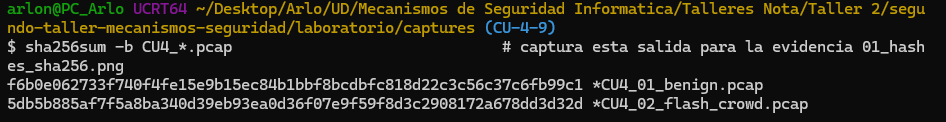
\includegraphics[width=0.92\textwidth]{imagenes/Evidencias CU-4/01_hashes_sha256.png}
\caption{Custodia e integridad de la evidencia del Caso 4.}
\label{fig:c4_hashes}
\end{figure}

\begin{figure}[H]
\centering
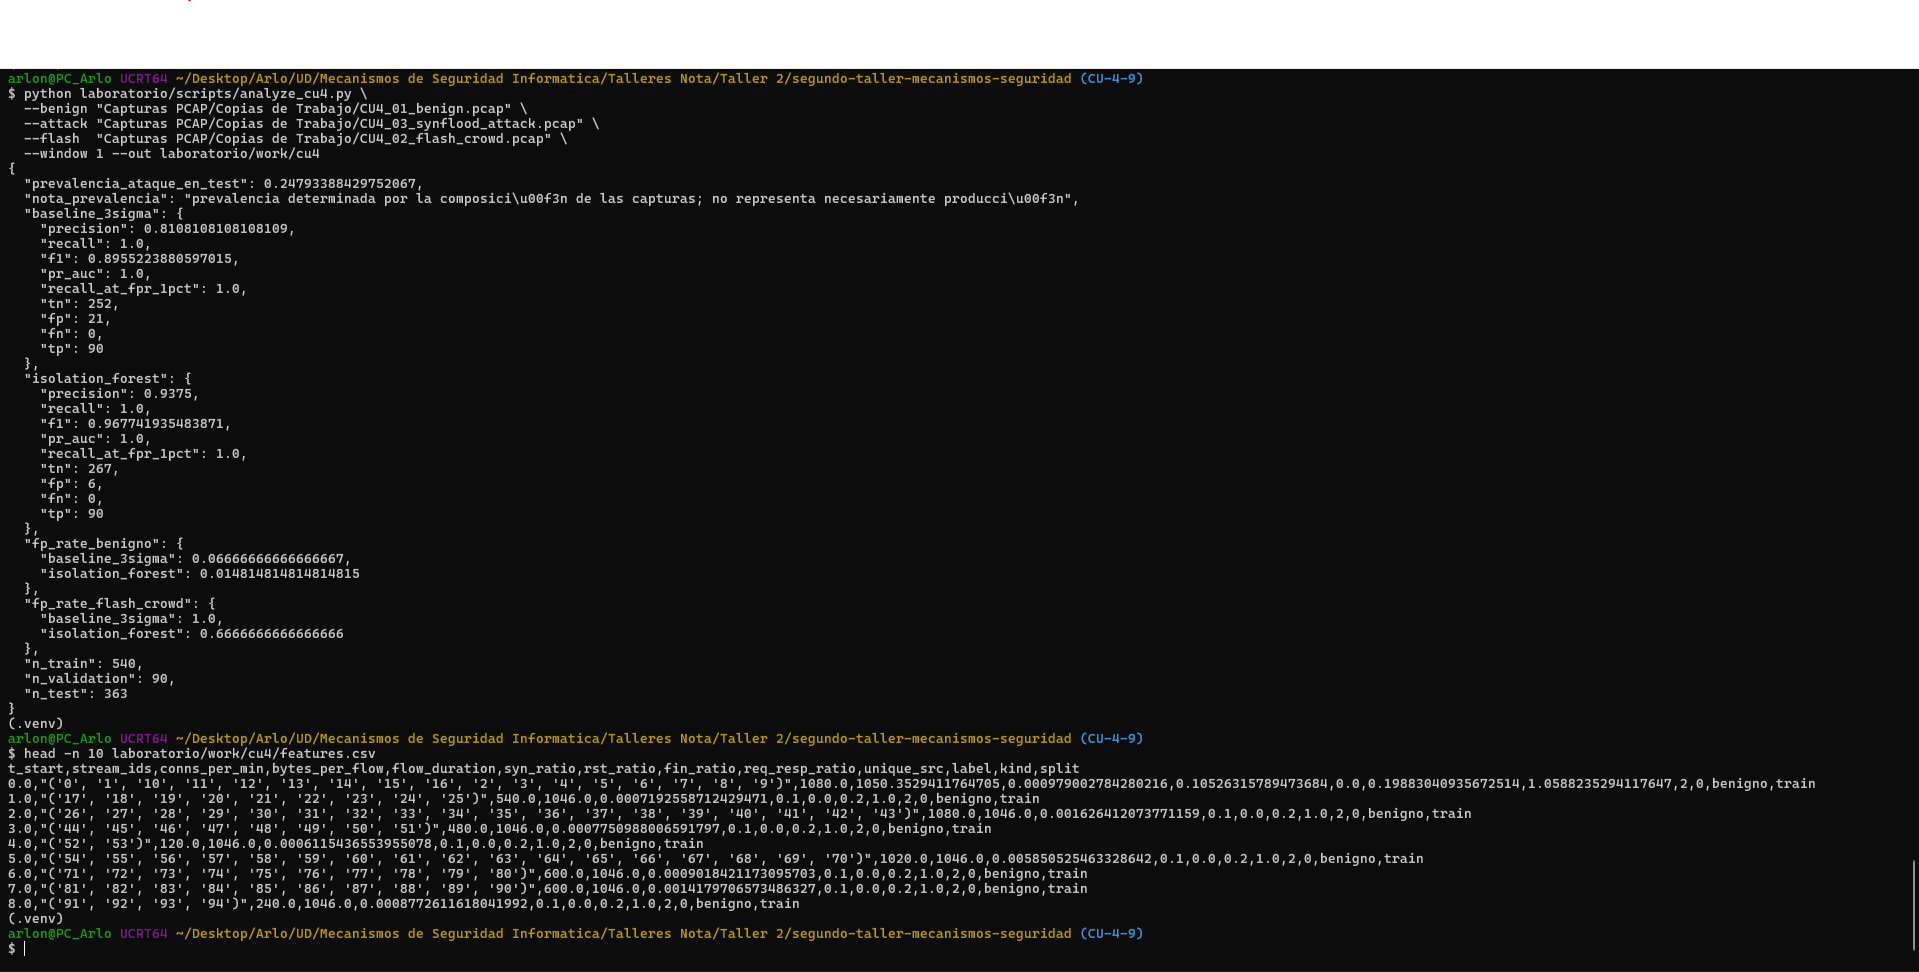
\includegraphics[width=0.92\textwidth]{imagenes/Evidencias CU-4/02_extraccion_atributos.png}
\caption{Extracción de atributos y agregación temporal del Caso 4.}
\label{fig:c4_atributos}
\end{figure}

\begin{table}[H]
\caption{Características agregadas para el detector de anomalías}
\label{tab:caracteristicas-ml}
\centering
\footnotesize
\renewcommand{\arraystretch}{1.25}
\begin{tabularx}{\textwidth}{@{}>{\raggedright\arraybackslash}p{0.25\textwidth} Y >{\raggedright\arraybackslash}p{0.16\textwidth} >{\raggedright\arraybackslash}p{0.12\textwidth}@{}}
\toprule
\textbf{Característica} & \textbf{Definición operativa en \texttt{window\_features}} & \textbf{Unidad} & \textbf{Ventana} \\
\midrule
Conexiones por minuto & \texttt{syn\_only / window * 60.0}; cuenta paquetes SYN sin ACK & SYN/min & \texttt{window} \\
Bytes por flujo & \texttt{g["bytes"].sum() / max(g["stream"].nunique(), 1)} & bytes/flujo & \texttt{window} \\
Duración del flujo & Media de \texttt{max(t) - min(t)} por cada \texttt{stream} en el grupo & segundos & \texttt{window} \\
Proporción SYN & \texttt{syn\_only / n} & razón & \texttt{window} \\
Proporción RST & \texttt{sum(rst) / n} & razón & \texttt{window} \\
Proporción FIN & \texttt{sum(fin) / n} & razón & \texttt{window} \\
Proporción petición/respuesta & \texttt{syn\_only / max(synack, 1)} & razón & \texttt{window} \\
Orígenes únicos & \texttt{g["src"].nunique()} & IPs únicas & \texttt{window} \\
\bottomrule
\end{tabularx}
\end{table}

\paragraph{Resultados obtenidos.}
El conjunto de prueba registró una prevalencia de ataque \texttt{prevalencia\_ataque\_en\_test}=0.2479 (24.79\,\%). Este valor describe la composición de las capturas evaluadas y no representa necesariamente la prevalencia de producción, tal como advierte la nota explicativa en el archivo de métricas.

\begin{table}[H]
\centering
\caption{Métricas de detección del Caso 4}
\label{tab:c4_metricas}
\footnotesize
\renewcommand{\arraystretch}{1.2}
\begin{tabularx}{\textwidth}{@{}l X r r@{}}
\toprule
\textbf{Métrica} & \textbf{Descripción} & \textbf{Línea base 3-sigma} & \textbf{Isolation Forest} \\
\midrule
Precisión & Proporción de predicciones anómalas correctas & 0.8108 & 0.9375 \\
Recall & Proporción de ataques detectados & 1.0000 & 1.0000 \\
F1 & Equilibrio armónico entre precisión y recall & 0.8955 & 0.9677 \\
PR-AUC & Área bajo la curva Precision--Recall & 1.0000 & 1.0000 \\
Recall al FPR 1\,\% & Recall garantizado al limitar FPR al 1\,\% & 1.0000 & 1.0000 \\
Verdaderos negativos & Ventanas normales clasificadas correctamente & 252 & 267 \\
Falsos positivos & Ventanas normales clasificadas como anómalas & 21 & 6 \\
Falsos negativos & Ataques no detectados & 0 & 0 \\
Verdaderos positivos & Ataques detectados correctamente & 90 & 90 \\
\bottomrule
\end{tabularx}
\end{table}

\begin{figure}[H]
\centering
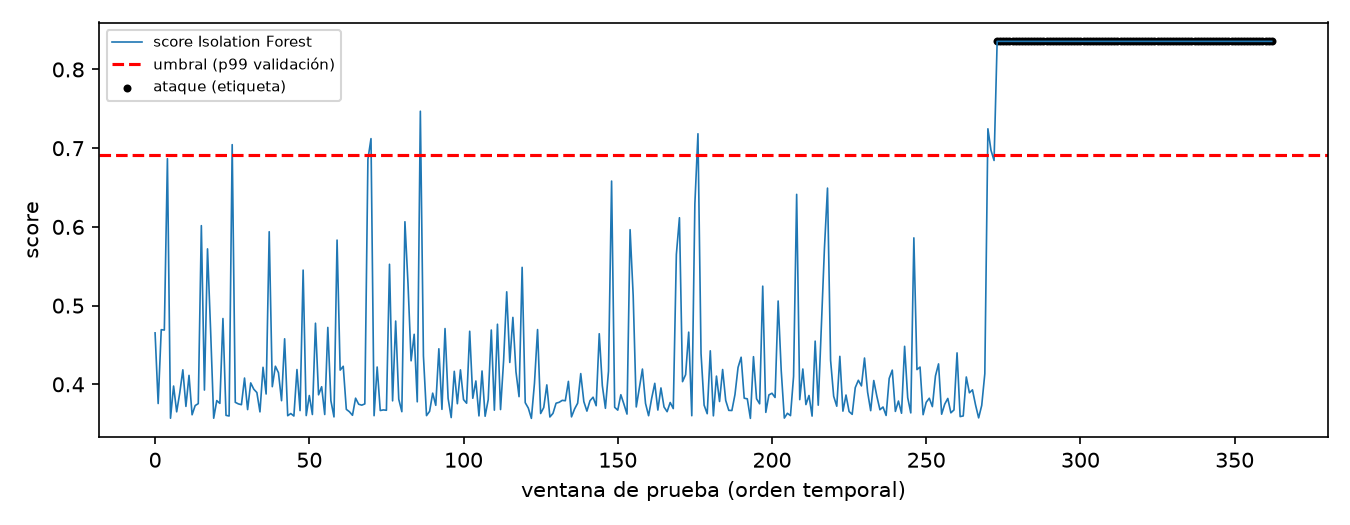
\includegraphics[width=0.95\textwidth]{imagenes/Evidencias CU-4/03_scores_iforest.png}
\caption{Puntuaciones del Isolation Forest y umbral calibrado.}
\label{fig:c4_scores}
\end{figure}

\begin{figure}[H]
\centering
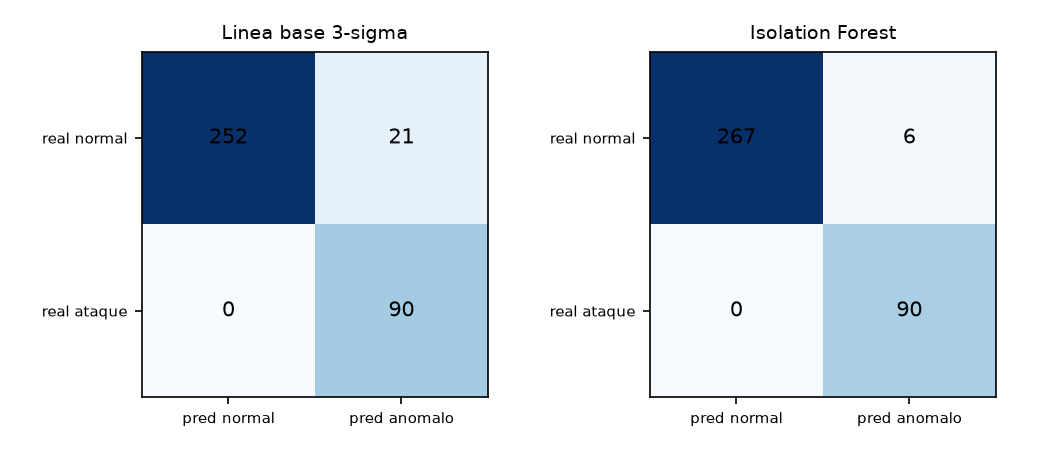
\includegraphics[width=0.90\textwidth]{imagenes/Evidencias CU-4/04_matrices_confusion.png}
\caption{Matrices de confusión de la línea base y Isolation Forest.}
\label{fig:c4_confusion}
\end{figure}

\begin{figure}[H]
\centering
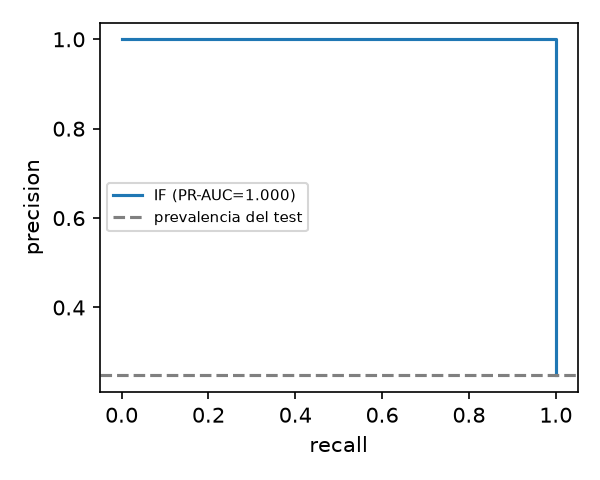
\includegraphics[width=0.72\textwidth]{imagenes/Evidencias CU-4/05_curva_pr.png}
\caption{Curva Precision--Recall del detector.}
\label{fig:c4_pr}
\end{figure}

\begin{figure}[H]
\centering
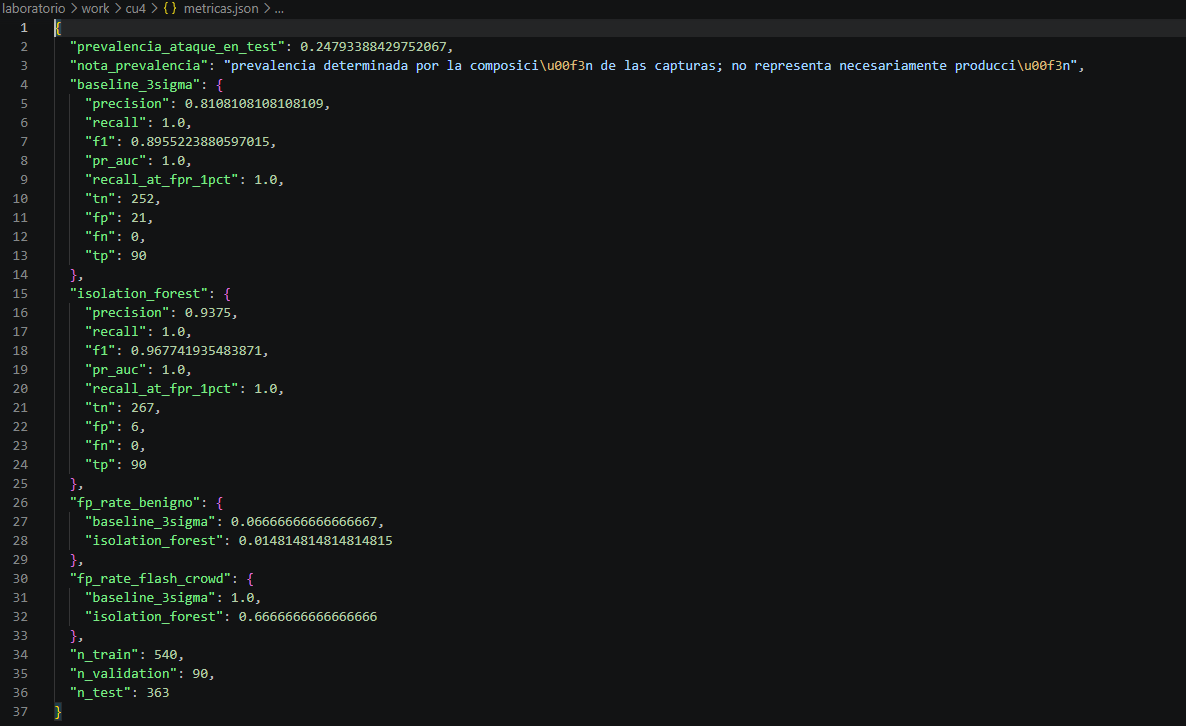
\includegraphics[width=0.95\textwidth]{imagenes/Evidencias CU-4/06_metricas_json.png}
\caption{Métricas serializadas del análisis del Caso 4.}
\label{fig:c4_metricas_json}
\end{figure}

Las tasas de falsos positivos por tipo de tráfico son las siguientes:

\begin{itemize}
\item \textbf{Tráfico benigno:} \texttt{fp\_rate\_benigno}=0.0667 (6.67\,\%) para la línea base y 0.0148 (1.48\,\%) para Isolation Forest.
\item \textbf{Ráfaga legítima:} \texttt{fp\_rate\_flash\_crowd}=1.0000 (100\,\%) para la línea base y 0.6667 (66.67\,\%) para Isolation Forest.
\end{itemize}

\paragraph{Análisis de resultados.}
La línea base estadística detectó todos los ataques registrados en la prueba (\texttt{recall}=1.0, \texttt{fn}=0), pero produjo 21 falsos positivos. Isolation Forest también detectó todos los ataques y redujo los falsos positivos a 6. Por ello, Isolation Forest presenta una puntuación F1 superior de 0.9677 frente al 0.8955 de la línea base.

El resultado no debe interpretarse como una garantía de operación perfecta: aunque ambos métodos obtuvieron \texttt{pr\_auc}=1.0, la tasa de falsos positivos en ráfagas legítimas (\texttt{fp\_rate\_flash\_crowd}=0.6667) demuestra que los incrementos súbitos de carga autorizada pueden simular un comportamiento anómalo. Esto refleja un fenómeno de deriva de concepto y justifica exigir persistencia en la detección y validación por analistas antes de aplicar mitigaciones automáticas.

\paragraph{Indicadores de detección.}
\begin{itemize}
\item \textbf{Desviación sostenida respecto a la línea base:} anomalía persistente durante varias ventanas consecutivas.
\item \textbf{\texttt{req\_resp\_ratio} alto:} desbalance significativo de paquetes SYN frente a respuestas SYN/ACK.
\item \textbf{\texttt{syn\_ratio} alto:} alta concentración de peticiones de apertura de conexión.
\item \textbf{\texttt{unique\_src} alto:} incremento en la diversidad de direcciones IP de origen.
\item \textbf{\texttt{bytes\_per\_flow} bajo:} flujos incompletos o de tamaño mínimo característicos de un escaneo o inundación.
\end{itemize}

\paragraph{Regla de detección propuesta.}
A partir del análisis volumétrico realizado con \texttt{case4\_max\_syn.sh} (donde el pico benigno fue de 72 SYN/5s, la ráfaga de 150 SYN/5s y el ataque de 758 SYN/5s), se establece un umbral operativo de **200 paquetes SYN en una ventana de 5 segundos** para la regla Suricata \texttt{sid:1004001}:

\begin{verbatim}
alert tcp any any -> $HOME_NET any (
  msg:"POSIBLE SYN FLOOD - Exceso de SYN en 5s (CU4)";
  flags:S,12;
  threshold: type threshold, track by_dst, count 200, seconds 5;
  sid:1004001; rev:1;
)
\end{verbatim}

La regla evalúa el destino (\texttt{track by\_dst}) para proteger a los servidores internos de saturaciones por inundación SYN, evitando falsos positivos durante ráfagas de tráfico legítimo menores a 150 SYN/5s. La validación en ejecución se presenta en la Figura~\ref{fig:c4_suricata}.

\begin{figure}[H]
\centering
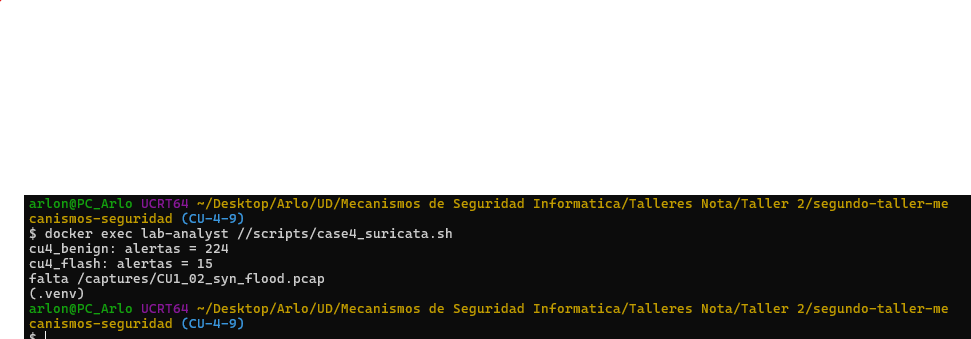
\includegraphics[width=0.95\textwidth]{imagenes/Evidencias CU-4/07_suricata_syn.png}
\caption{Alertas de Suricata asociadas al Caso 4.}
\label{fig:c4_suricata}
\end{figure}

\paragraph{Mitigación y defensa.}
\begin{itemize}
\item \textbf{Revisión humana:} mantener supervisión activa en el SOC; no automatizar bloqueos definitivos basados únicamente en puntuaciones de modelos de aprendizaje automático.
\item \textbf{Monitorización de deriva:} supervisar periódicamente las métricas \texttt{fp\_rate\_benigno} y \texttt{fp\_rate\_flash\_crowd} frente a cambios de patrón de tráfico.
\item \textbf{Protección de los datos de entrenamiento:} resguardar la integridad de los datasets de entrenamiento para evitar ataques de envenenamiento o fuga de datos.
\item \textbf{Calibración periódica:} reajustar el percentil 99 de corte al incorporar nuevos patrones de tráfico legítimo.
\item \textbf{Defensa en profundidad:} correlacionar las alertas del IDS Suricata con los eventos del WAF y registros del servidor web.
\end{itemize}

\paragraph{Preguntas de análisis.}
\begin{enumerate}[leftmargin=*, topsep=2pt, itemsep=2pt]
\item \textbf{¿Cómo afectan el desbalance de clases y los cambios legítimos de carga?}\par
Con una prevalencia de prueba del 24.79\,\%, la precisión y la PR-AUC deben evaluarse conjuntamente con el comportamiento frente a cargas legítimas. La ráfaga produce un 66.67\,\% de falsos positivos en Isolation Forest, lo que evidencia que el aumento de volumen sin contexto puede confundirse con una anomalía maliciosa.
\item \textbf{¿Qué métrica es más útil para este caso?}\par
El recall por sí solo no basta (1.0000 en ambos modelos). La combinación más representativa está dada por el F1-score (0.9677), la curva PR-AUC y la tasa de falsos positivos desglosada por tipo de tráfico (\texttt{fp\_rate\_flash\_crowd}).
\end{enumerate}

\paragraph{Conclusiones.}
\begin{itemize}
\item Ambos modelos lograron un recall del 100\,\% (\texttt{recall}=1.0, \texttt{tp}=90, \texttt{fn}=0).
\item Isolation Forest redujo los falsos positivos a 6 frente a los 21 registrados por la línea base estadística de $3\sigma$.
\item Las ráfagas autorizadas representan el principal factor de falsos positivos en modelos no supervisados por volumen.
\item La regla de Suricata calibrada en 200 SYN/5s permite filtrar la ráfaga de carga (150 SYN/5s) detectando eficazmente el SYN flood (758 SYN/5s).
\end{itemize}

\begin{table}[H]
\centering
\caption{Ficha de registro del hallazgo. Caso 4}
\label{tab:ficha-c4}
\footnotesize
\renewcommand{\arraystretch}{1.2}
\begin{tabularx}{\textwidth}{@{}>{\raggedright\arraybackslash}p{0.23\textwidth} Y@{}}
\toprule
\textbf{Campo} & \textbf{Registro} \\
\midrule
Identificador & Caso 4 - Detección de anomalías en tráfico TCP/IP. Analista: Arlo Nicolás Ocampo Gallego. \\\hline
Fecha y hora & Noviembre 2026; evidencia registrada en \texttt{laboratorio/work/cu4/metricas.json}. \\\hline
Origen/destino & Red de laboratorio de pruebas (\texttt{172.28.50.0/24}). \\\hline
Observación & Isolation Forest obtiene $F_1=0.9677$ con 6 falsos positivos en el test set, superando el modelo $3\sigma$ (21 FP). \\\hline
Hipótesis & Un incremento en \texttt{syn\_ratio} y desbalance en \texttt{req\_resp\_ratio} identifica un ataque SYN Flood, aunque ráfagas legítimas pueden generar falsos positivos temporales. \\\hline
Validación & Archivo \texttt{metricas.json}, matrices de confusión y alertas de la regla Suricata 1004001 en la Figura~\ref{fig:c4_suricata}. \\\hline
Severidad & Alta (Detección de denegación de servicio por agotamiento de recursos). \\\hline
Acción & Aplicar rate-limiting, requerir ventana de persistencia y mantener supervisión humana en el SOC. \\\hline
Integridad & SHA-256 verificado en la Figura~\ref{fig:c4_hashes}. \\
\bottomrule
\end{tabularx}
\end{table}